 \documentclass[onecolumn]{aastex63}
\usepackage{amsmath}
\usepackage{listings}
\usepackage[T1]{fontenc}
\newcommand{\vdag}{(v)^\dagger}
\newcommand\aastex{AAS\TeX}
\newcommand\latex{La\TeX}
\newcommand\lya{Ly$\alpha$\ }
\shortauthors{McClellan}
\graphicspath{{./}{figures/}}

\begin{document}

\title{Exoplanet Atmospheres through Hubble's Cosmic Origins Spectrograph}
\author{B. Connor McClellan}
\affiliation{University of Virginia}
\keywords{}

\begin{abstract}
    UV irradiation of exoplanets near the parent star can heat and ionize hydrogen-rich upper atmospheres, producing a pressure-driven outflow that can exceed the Roche lobe of the planet. This extended atomic hydrogen atmosphere has been observed in UV wavelengths by the Hubble Space Telescope for several planets. In one particular case, the line is blue-shifted, indicating that Lyman alpha radiation forces have accelerated hydrogen atoms away from the star to large velocities. Though the presence of these extended clouds are strongly suspected, their extent over the planet's orbit has not been fully characterized. Follow-up observations with Hubble's Cosmic Origins Spectrograph can deliver high-resolution transit depths and light curves across the FUV and NUV bands, which will reveal the temperature, density, dynamics, and composition of the atmospheres of distant worlds.
    \vspace{1cm}
\end{abstract}

\section{Motivation}
Exoplanet transit spectroscopy has the potential to reveal the contents of the atmospheres of distant worlds. As starlight filters through the exoplanet's atmosphere, molecular and atomic species absorb specific frequencies of photons due to their electron configurations, leaving a fingerprint on the light that reaches the observer. Based on the width and depth of these absorption lines, one can discern the temperature and particle density of the atmosphere as well. The opacity of this material can depend strongly on the wavelength of light passing through it, meaning some frequencies are particularly well-suited for studying high altitude atmospheric dynamics and abundances. In particular, the stellar Lyman Alpha (\lya) line interacts most strongly with the lowest density planetary gas, making it much better for calculating very small pressure gradients than optical and infrared observations.

In previous observations by Hubble (discussed in section 2), it was shown that stellar UV irradiation of several exoplanets' atmospheres drives an outflow that produces a large exospheric cloud of weakly-bound atoms; in some cases, the cloud extends out near the Roche lobe, suggesting atmospheric escape. The atoms which are accelerated by this radiation are embedded in the gas surrounding the planet, such that collisions with protons will limit the atoms' acceleration by stellar radiation. 

The center of the \lya line is obfuscated by absorption in the interstellar medium and geocoronal emission. However, \lya photons with frequencies at line center are doppler shifted by the planet's orbital motion, and are therefore observable even from Earth. Due to the extended nature of the cloud, this means line center \lya can be observed \textit{outside of the transit window} which could reveal the boundary between low-density planetary gas and the stellar wind from the host star. The extent of the cloud along the planet's orbit has not been quantified, yet Ehrenreich et al. (2015) guess that it could last up to 20 hours after the optical transit. Hubble's Cosmic Origins Spectrograph has the spectral resolution to characterize this phenomenon more effectively than previous studies. Light curves and transit depths can reveal the nature and extent of this radiation-driven outflow.

Lyman Alpha is not the only transition of note in such systems. However, it is the strongest line and the most abundant species present, so it is a paragon for the irradiation of exoplanetary atmospheres by starlight. Other atomic lines from less abundant species are produced at layers deeper in the atmosphere than \lya, which leads to smaller overall transit depths. Such absorption has been detected for Na, O, C+, Mg, Si++, and H for the H$\alpha$, H$\beta$, and H$\gamma$ lines. Here, the physics becomes slightly more complicated; if the lower state of the atomic transition is not the ground state, the state will be unpopulated in the absence of collisional or radiative excitation. Thus, these particular transitions depend sensitively on the temperature and radiation present deeper into the atmosphere. Some elements have been predicted to have large optical depths which haven't been observed in transit (Turner et al. 2016), and non-detections of these elements can constrain the atmospheric structure and abundances further. This is yet another opportunity for Hubble COS to shine.

The outer layers of planetary atmospheres are central to a planet's evolution, as they can shelter the lower atmosphere from high energy radiation and regulate the escape of gas into space. Planets that are close to their parent stars produce transits for a larger portion of the sky. This means that, observing from Earth, we tend to observe transits of planets that are subjected to large amounts of radiation and stellar wind fluxes. With observations of these close-in systems, we can explore fundamental questions about the evolution and stability of their atmospheres, examining which physical and chemical processes are important and characterizing the rate of atmospheric mass loss. From atomic data, opacities, and stellar optical-EUV spectra, one can construct a model of this behavior for large optical depths and obtain radiation pressure forces, excitation, heating, and cooling, among other valuable properties to explain the phenomenon.
 
\section{RECENT WORK}

Hubble Space Telescope (HST) observations with STIS have found large Lyman $\alpha$ transit depths around the gas giants HD 209458b \citep{2003Natur.422..143V}, HD 189733b \citep{2012A&A...543L...4L} and 55 Cnc b \citep{2012A&A...547A..18E}, Neptune-size planets GJ 436 b 
\citep{2015Natur.522..459E}
and GJ 3470 b \citep{2018A&A...620A.147B}, and possibly the super-Earth HD 219134b \citep{2019EPSC...13.1928L}. In the case of GJ 436 b, ultraviolet transit depths of 56\% are reported, claiming a total Ly-$\alpha$ eclipse would have been possible for a central transit. Notably, the most notable absorption occurs in the blue wing of the Ly-$\alpha$ line. Non-detections or marginal detections have been reported for the super-Earths 55 Cnc e \citep{2012A&A...547A..18E}, super-Earth HD 97658 b \citep{2017A&A...597A..26B} , super-Earth GJ 1132 b \citep{2019AJ....158...50W}, super-Earth $\pi$ Men c \citep{2020ApJ...888L..21G}, and marginal detections were Earth-size TRAPPIST-1 \citep{2017A&A...599L...3B} and sub-Earth Kepler-444 \citep{2017A&A...602A.106B}. Observations of GJ 436b show blue-shifted absorption, possibly due to acceleration of the planet’s atmosphere by radiation pressure from the star. \cite{2021ApJ...907L..36M} reports a detection of CII ions in a single transit of the exoplanet $\pi$ Men c, with transit depths and Doppler velocities consistent with an escaping atmosphere. The paper claims their findings confirm the hypothesized compositional diversity of small exoplanets. 

These observations for transiting planets have revealed a population of atoms extending out to distances of order the planetary radius for several planets around bright, nearby stars. Extended atmospheres of irradiated exoplanets can be used to probe the deeper layers of the planet. In the case of HD 209458b, observations detected atomic hydrogen (H) absorption in the stellar Ly-$\alpha$ line during three transits. Observational data was taken from the Space Telescope Imaging Spectrograph (STIS) onboard the Hubble Space Telescope (HST) using the G140M grating to minimize contamination from Earth's Ly-$\alpha$ geocoronal emission. The remaining geocoronal emission was removed by subtracting the sky spectrum from the stellar spectrum (possible because the sky spectrum fulls the entire aperture of the spectrograph). Two separate methods for dark-subtraction were used, both converging at the same result with low systematic errors. The planet's radius and mass suggest the absorption takes place beyond the Roche limit (i.e., the absorption is occurring in escaped H atoms). The magnitude of absorption is larger than it should be for a planet occulting 1.5\% of the star's visible surface. A maximally-filled Roche lobe would account for only 10\% absorption. The outlying 5\% suggests that hydrogen is escaping the planet's atmosphere. Models designed by the authors suggest that the escaping hydrogen atoms expand in an asymmetric comet-like tail and progressively disappear when moving away from the planet, which is consistent with observations. The absorption is thought to last well after the end of the transit due to the large physical size of the evaporating tail. In this way, mass and radius measurements allow advanced analysis to be done on Ly-$\alpha$ spectral features, as it is possible to discern what fraction of the absorbing atoms are gravitationally bound to the planet. It has been determined observationally that HD209458b is evaporating, producing a streaming tail of escaping hydrogen atoms.

\newpage

\section{OBSERVATIONAL DIAGNOSTICS}

The observed spectra are expected to be typical for a solar-type star, with a double-peaked emission originating from the stellar chromosphere. The central absorption feature should be wide due to neutral hydrogen in the interstellar medium. As seen in \cite{2003Natur.422..143V}, the geocoronal emission will almost certainly fill the aperture of the spectrograph, resulting  in  an  extended emission line perpendicular to the dispersion direction. Thankfully, this means it is easy to remove at the position of the target star. The COS pipeline should extract 1D spectra from which the background has not been removed. Thus, the background can be fit in 1D and subtracted from the target spectra.

\begin{figure}
    \centering
    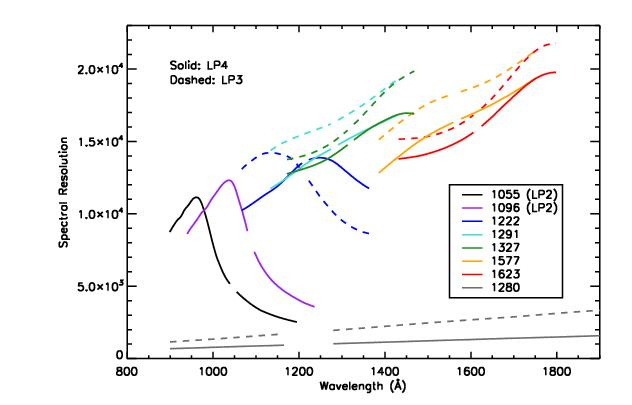
\includegraphics{spec.jpg}
    \caption{Resolving Power for FUV gratings.}
    \label{fig:my_label}
\end{figure}

The COS medium-resolution channels can be used to achieve a wavelength accuracy of 15 km s$^{-1}$, which is more than enough to resolve the spectral features we are looking for in this study. The FUV channel has a cross delay line (XDL) detector consisting of two 16384 $\times$ 1024 pixel segments. The segments are separated by a gap of 9 mm, and the central wavelength positions of the instrument were selected to enable full wavelength coverage of this gap. Positions of wavelength coverage for each grating setting is shown in Fig \ref{fig:my_label}.

In order to quantify transit depths for \lya, Na, O, C+, Mg, Si++, H$\alpha$, H$\beta$, and H$\gamma$ lines, combinations of gratings and central wavelength settings must be chosen for optimal coverage of lines. Table \ref{tab:my_label} shows an example of these selections made for the Lyman Alpha line. Since the other lines of Hydrogen are not observable in the UV, they will not be included in this study.

\begin{table}[]
    \centering
    \begin{tabular}{lrlr}
        Line & Wavelength (angstroms) & Grating & Central Wavelength \\
        \hline
        \lya & 1219 & G130M & 1291\\
    \end{tabular}
    \caption{Example grating and central wavelength selections for Lyman Alpha. Identification of lines of interest for other species will follow the same procedure.}
    \label{tab:my_label}
\end{table}


\newpage
\section{PROPOSED TELESCOPE SETUP}

Both light-curves and spectra are important to understanding the dynamics within these systems. A single transit may be observed for several hours to determine the extent of the hydrogen cloud around the planet. The G130M grating will be used with a central wavelength setting of 1291 angstroms, which will cover the Lyman Alpha line. Follow-up studies can be repeated following the same procedure for other species and transitions, with exposure times adjusted to reflect their relative transit depths.

Following the motivations in \cite{2003Natur.422..143V}, consecutive HST orbits will be scheduled  such  that  the  first  orbit  (~900 s  exposure)  ends 2 hours before the first contact of the planet with the stellar disk. Exposures will be scheduled as often as Hubble's orbit allows to provide a baseline upon which a rough time series can be built. Upon contact with the stellar disk, the exposures will lengthen to ~2,100 s to increase the throughput and lower Poisson noise. After the transit is completed, more 900 s exposures will be taken for at least 20 hours, to confirm when the trail of escaping hydrogen from the planet completes its transit. This will finally confirm the true extent of the escaping hydrogen cloud via transit spectroscopy, allowing particle densities and temperatures to be derived at each point during the transit.

\bibliography{bibliography}{}
\bibliographystyle{aasjournal}

\end{document}